\documentclass[11pt,letterpaper]{article}
\usepackage[T1]{fontenc}
\usepackage[utf8]{inputenc}
\usepackage{iftex}
\ifPDFTeX
\usepackage{mathptmx}
\else
\usepackage{fontspec}
\IfFontExistsTF{Times New Roman}{\setmainfont{Times New Roman}}{\setmainfont{TeX Gyre Termes}}
\fi
\usepackage[margin=1in]{geometry}
\usepackage{graphicx,longtable,array,setspace,multicol}
\usepackage[hidelinks]{hyperref}
\usepackage{caption}
\setlength{\parindent}{0pt}
\setlength{\parskip}{6pt}
\setlength{\emergencystretch}{3em}
\captionsetup{font=small,labelfont=bf}
\pagestyle{plain}
\begin{document}
\begin{center}{\Large\bfseries Stop Overthinking, Keep Passing the Tests}\par\medskip Shortest Correct LoRA Training and Free Thinking Controls in Small Qwen3.5 Code Models\par\medskip [AUTHOR NAME]\\{}[DEPARTMENT], [UNIVERSITY]\\{}[EMAIL]\end{center}
\begin{multicols}{2}


\section*{Abstract}\addcontentsline{toc}{section}{Abstract}

Small language models can generate long reasoning traces without completing correct code. We compare shortest-correct low-rank adaptation training with thinking controls in Qwen3.5-0.8B, 2B, and 4B. The retrospective evaluation combines saved grades for 464 problems: 164 HumanEval+ and 300 LiveCodeBench tasks. Historical summaries average attempts within each problem, while completed-control comparisons separately use first attempts. All six trained combinations with thinking OFF or selected thinking limits are complete. LoRA plus OFF passes 65, 165, and 300 problems; LoRA plus limits passes 67, 191, and 332. The 2B limit combination reaches 41.2\%, but its gain over the matching free limit remains uncertain. The 4B combination reaches 71.6\%, with an uncertain accuracy change and about 11.4\% fewer output tokens than the free-limit first attempt. These findings support testing strong free controls before investing in this training procedure. Results are limited by retrospective selection, historical environments, unadjusted intervals, and grading scope.\par

Keywords: code generation; efficient reasoning; thinking budget; LoRA; Qwen3.5.\par

\section*{1 Introduction}\addcontentsline{toc}{section}{1 Introduction}

Efficient code generation requires correct programs as well as controlled output. Explicit reasoning can help a model plan, but it can also repeat notes or consume the output space needed for code. The efficient-reasoning literature motivates interventions on this tradeoff \cite{survey}. The practical question in this paper is whether a trained concise-reasoning add-on provides a useful advantage beyond the inference controls already available to a small model.\par

We study Qwen3.5-0.8B, 2B, and 4B \cite{q08,q2,q4}. A free control means a policy that requires no additional training. It does not mean generation is computationally free. The controls are unrestricted explicit thinking, thinking OFF, and selected thinking-token limits. We also evaluate saved LoRA-1 add-ons alone and in combination with OFF or a limit.\par

The distinction between a weak reference and a matching control is central. A trained model with limited thinking may beat an untrained model with unrestricted thinking because the limit itself is helpful. To evaluate the added value of training, the trained limited model should also be compared with the same limit without training. Similarly, a trained OFF configuration needs an untrained OFF reference.\par

Our contributions are a unified account of a completed three-size study, an explicit separation of attempt rules, and matched comparisons for all six trained controls on 464 shared problem IDs. The study is empirical and retrospective. It introduces neither a new model architecture nor a claim that these policies are optimal outside the measured setting.\par

\section*{2 Background and Related Work}\addcontentsline{toc}{section}{2 Background and Related Work}

LoRA freezes pretrained weights and learns low-rank update matrices \cite{lora}. It provides an economical adaptation mechanism, but the quality of the learned behavior still depends on the supervision. In this study, shortest-correct selection generates several practice answers, retains a successful short target where available, and trains an add-on from those examples.\par

Self-training with concise reasoning motivates this procedure \cite{selftrain}. SEER studies compression through self-generated data and filtering in software engineering \cite{seer}, while ASAP uses anchor-guided and surprisal-based pruning \cite{asap}. These interventions are related to the present goal but differ in model scale, training data, and selection method. Their reported reductions are not predictions for this experiment.\par

Thinking controls provide a competing route. NoThinking motivates direct answering under constrained reasoning budgets \cite{nothink}. The s1 work includes interventions that terminate or extend explicit reasoning \cite{s1}. These sources justify including simple controls rather than treating unrestricted thinking as the only reference.\par

For code evaluation, EvalPlus strengthens functional checking with extended tests \cite{evalplus}. LiveCodeBench supplies contest-based tasks over time \cite{lcb}. MBPP provides function-level programming material \cite{mbpp}; its extended version is used here for training, not as part of the main test denominator. The paper reports success under the saved tests actually used, rather than formal program correctness.\par

\section*{3 Study Design}\addcontentsline{toc}{section}{3 Study Design}

\subsection*{3.1 Evidence and Test Collection}\addcontentsline{toc}{subsection}{3.1 Evidence and Test Collection}

The analysis reads saved outputs, settings, and grades. The document build performs no model training, answer generation, or execution of generated programs. The test collection contains 164 HumanEval+ tasks, 166 LiveCodeBench easy tasks, and 134 medium tasks. There are no hard contest tasks. Unique IDs permit matching across configurations and structural overlap checks.\par

The collection grew from an original 234 problems through later groups of 40 and 190. The combined view was chosen after results were available. It should therefore be interpreted as a retrospective summary of accumulated evidence, not a newly preregistered exam. Some exploratory methods remain partial, and their scores are excluded from full-coverage rankings.\par

HumanEval+ uses extended evaluation tests. The saved LiveCodeBench grader uses up to 20 tests per problem. An answer passes only if the extracted program passes all tests actually used for that attempt. This operational definition is narrower than success on every hidden test in the benchmark or on every possible input.\par

\subsection*{3.2 Training and Controls}\addcontentsline{toc}{subsection}{3.2 Training and Controls}

LoRA-1 uses a pool of 100 easy function problems and selects successful practice answers for training. The available short successful targets depend on the model. The historical LoRA-2 experiment uses a different 280-problem pool, retains 157 examples, and covers the original 234 test problems. It is kept separate from the full-set LoRA-1 comparisons.\par

Thinking ON permits explicit notes until stopping or the overall cap. OFF requests a direct answer. A thinking limit ends the notes at a budget and then allows the answer. Selected budgets are 512 tokens for 0.8B, 1,024 for 2B, and 2,048 for 4B. These are thinking budgets, not total-output caps. LoRA alone means the trained add-on with thinking ON and no additional limit.\par

Sampling records temperature 0.6, top-p 0.95, top-k 20, and seed 3407. Total-output caps are 4,096 tokens for HumanEval+ and 8,192 for LiveCodeBench. Repeat stopping is enabled in the 0.8B and 4B extensions; 2B retains its original handling. Historical references use earlier packages and batch layouts, so the cross-size comparison is not a controlled change in model scale alone.\par

The completed-control environment records Python 3.13.15, PyTorch 2.9.1 with CUDA 12.8, Transformers 5.18.0, and PEFT 0.21.1, with bfloat16 calculations. Notebook 24 records an A100 80GB accelerator. These details identify the extension environment rather than implying uniform conditions across every historical run.\par

\subsection*{3.3 Estimators and Uncertainty}\addcontentsline{toc}{subsection}{3.3 Estimators and Uncertainty}

For the historical combined view, accuracy is the mean of each problem's fraction of passing attempts. This gives each problem equal weight even when attempt counts differ. For example, one pass from two attempts contributes 0.5, while one pass from one contributes 1.0. Pooling every attempt would instead give more influence to repeatedly sampled problems.\par

Each completed combination has one attempt on all 464 problems. Its matched-control analysis uses the saved first attempt of the historical reference on the same IDs. This view is labeled separately. The 4B free limit is 71.9\% in the all-attempt summary and 71.1\% in the first-attempt reference; these are different estimators rather than inconsistent rounding.\par

Differences use paired problem bootstrap intervals with 2,000 replicates and seed 3407. Each sampled ID retains both methods. Intervals are percentile 95\% intervals, unadjusted for multiple comparisons or retrospective selection. They represent variation over the observed problem collection, not every source of generation, training, or deployment uncertainty.\par

Missing results are never scored as failures. A partial method's denominator is its covered set, and a direct comparison uses shared IDs. This prevents a strong score on a smaller subset from being presented as a superior complete-set result. Coverage is a property of the evidence, not an accuracy metric.\par

\section*{4 Results}\addcontentsline{toc}{section}{4 Results}

\subsection*{4.1 Full Coverage Overview}\addcontentsline{toc}{subsection}{4.1 Full Coverage Overview}

Figure \ref{fig:conferenceXaccuracy} compares the selected free controls and trained limits using the all-attempt rule. The best observed full-coverage free scores are 14.7\% for 0.8B OFF, 38.6\% for 2B limit 1,024, and 71.9\% for 4B limit 2,048. Their unrestricted-thinking references score 4.1\%, 26.8\%, and 50.0\%. Thus unrestricted thinking is not the strongest available reference in this collection.\par

\begin{center}\begin{minipage}{\linewidth}\centering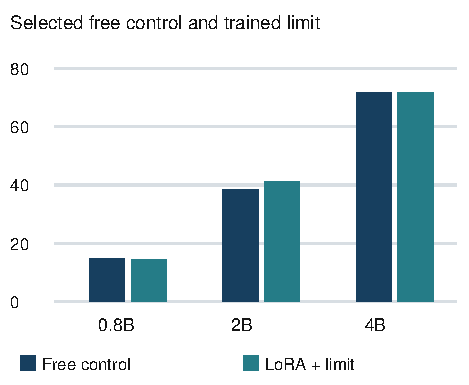
\includegraphics[width=\linewidth]{figures/conference_accuracy.pdf}\captionof{figure}{All-attempt accuracy on 464 problems. The selected free policy is OFF for 0.8B and a limit for 2B and 4B. The trained policy uses each size's selected limit.}\label{fig:conferenceXaccuracy}\end{minipage}\end{center}

LoRA alone scores 12.3\%, 34.4\%, and 56.8\% in the all-attempt view. The selected free controls score above these values on the shared 464 problems. The saved gap interval crosses zero for 0.8B, while the 2B and 4B all-attempt intervals favor the selected free controls. These are retrospective comparisons and do not establish the failure of all possible LoRA training designs.\par

\subsection*{4.2 Completed Trained Policies}\addcontentsline{toc}{subsection}{4.2 Completed Trained Policies}

Table \ref{tab:completed} reports all six completed combinations. Each row has one answer per problem. The 2B trained limit achieves 191/464, or 41.2\%, the highest observed complete-set 2B point estimate among the tested methods. The 4B trained limit reaches 332/464, or 71.6\%. Counts, coverage, intervals, and tokens should be read together rather than as an unlabeled ranking.\par

\end{multicols}
\begin{center}\begin{minipage}{\textwidth}
\begingroup\singlespacing\small\setlength{\tabcolsep}{4pt}
\captionof{table}{All six completed combinations with one answer per problem}\label{tab:completed}
\begin{tabular}{|p{0.913in}|p{0.913in}|p{0.913in}|p{0.913in}|p{0.913in}|p{0.913in}|}
\hline
\textbf{Size} & \textbf{Combination} & \textbf{Passed} & \textbf{Accuracy} & \textbf{95\% interval} & \textbf{Tokens}\\\hline
0.8B & LoRA + OFF & 65/464 & 14.0\% & [11.0\%, 17.0\%] & 1,278\\\hline
0.8B & LoRA + Limit  512 & 67/464 & 14.4\% & [11.2\%, 17.5\%] & 4,979\\\hline
2B & LoRA + OFF & 165/464 & 35.6\% & [31.2\%, 39.7\%] & 1,445\\\hline
2B & LoRA + Limit  1024 & 191/464 & 41.2\% & [36.6\%, 45.7\%] & 4,072\\\hline
4B & LoRA + OFF & 300/464 & 64.7\% & [59.9\%, 69.0\%] & 882\\\hline
4B & LoRA + Limit  2048 & 332/464 & 71.6\% & [67.5\%, 75.6\%] & 3,511\\\hline
\end{tabular}
\endgroup
\end{minipage}\end{center}
\begin{multicols}{2}

For 0.8B, untrained OFF passes 68/464, slightly more than either trained combination. The trained limit passes 67 compared with 49 for the free limit, an advantage of 3.9 points with an interval of +0.6 to +7.1. It therefore improves on that limited baseline without establishing an advantage over the stronger OFF option.\par

\subsection*{4.3 Matched First Attempts}\addcontentsline{toc}{subsection}{4.3 Matched First Attempts}

Table \ref{tab:first} and Figure \ref{fig:conferenceXforest} isolate the added training component relative to the same free policy. For 2B, LoRA plus limit exceeds the free limit by 2.6 points, with an interval from -1.5 to +6.7. The interval includes zero. The combination's higher observed score is therefore not an established accuracy gain over that reference.\par

\end{multicols}
\begin{center}\begin{minipage}{\textwidth}
\begingroup\singlespacing\small\setlength{\tabcolsep}{4pt}
\captionof{table}{Training addition versus the matching free policy on first attempts}\label{tab:first}
\begin{tabular}{|p{1.130in}|p{1.130in}|p{1.130in}|p{1.130in}|p{1.130in}|}
\hline
\textbf{Size / policy} & \textbf{Trained} & \textbf{Free} & \textbf{Gap pp} & \textbf{95\% gap pp}\\\hline
0.8B OFF & 14.0\% & 14.7\% & -0.6 & [-3.2, 2.2]\\\hline
0.8B limit & 14.4\% & 10.6\% & +3.9 & [0.6, 7.1]\\\hline
2B OFF & 35.6\% & 32.5\% & +3.0 & [-0.6, 6.9]\\\hline
2B limit & 41.2\% & 38.6\% & +2.6 & [-1.5, 6.7]\\\hline
4B OFF & 64.7\% & 66.4\% & -1.7 & [-5.6, 1.9]\\\hline
4B limit & 71.6\% & 71.1\% & +0.4 & [-3.0, 3.7]\\\hline
\end{tabular}
\endgroup
\end{minipage}\end{center}
\begin{multicols}{2}

For 4B, the free-limit first attempt passes 330 problems and the trained limit passes 332. The gap is approximately +0.4 points, with an interval of -3.0 to +3.7. This does not demonstrate a gain or practical equivalence. For OFF, the trained policy does not consistently improve accuracy across sizes. All three corresponding intervals include zero.\par

\begin{center}\begin{minipage}{\linewidth}\centering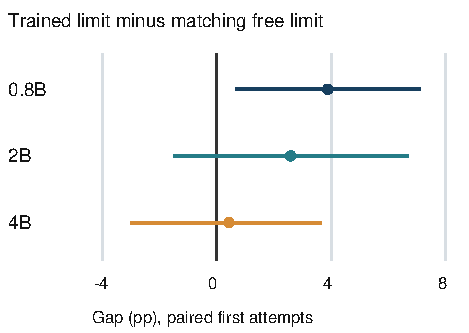
\includegraphics[width=\linewidth]{figures/conference_forest.pdf}\captionof{figure}{Matched first-attempt limit comparisons on 464 problems. Bars are unadjusted 95\% paired intervals; the 2B and 4B intervals cross zero.}\label{fig:conferenceXforest}\end{minipage}\end{center}

The 2B trained limit also beats trained OFF by 5.6 points, with an interval of +1.1 to +9.9. That comparison supports a role for the inference policy when using the saved add-on. It does not independently establish that training was necessary, since both compared systems contain the add-on.\par

\subsection*{4.4 Output Length and Historical Diagnostics}\addcontentsline{toc}{subsection}{4.4 Output Length and Historical Diagnostics}

Among the main free controls, OFF uses the fewest output tokens at each model size. In the all-attempt view, the 0.8B, 2B, and 4B OFF means are about 1,781, 1,337, and 943 total tokens. A thinking limit may improve accuracy while still producing longer complete answers, because its budget concerns the notes rather than the entire response.\par

For the 4B first-attempt limit comparison, the trained model averages about 3,511 tokens versus about 3,961 for the free reference, a reduction of approximately 11.4\%. This accompanies the uncertain accuracy difference. It is a measured token reduction and is not converted into an equal percentage reduction in time, energy, or money.\par

The historical 234-problem 2B study reports 190/468 cap hits for ON and 192/468 for LoRA-2. Among capped attempts, 69.5\% and 88.5\%, respectively, meet its loop rule. These percentages have different denominators from the cap rates and do not estimate looping on all 464 problems. The original LoRA-2 thinking-length ratio is 1.00 with an interval of 0.94 to 1.06, showing no observed shortening in that analysis.\par

\section*{5 Discussion and Limitations}\addcontentsline{toc}{section}{5 Discussion and Limitations}

The main practical lesson is to evaluate the simple policy that competes with the proposed training intervention. A large gain over unrestricted thinking can coexist with an uncertain difference from a free limit. This changes the decision about collecting practice candidates, training an add-on, and maintaining an adapted checkpoint.\par

A plausible mechanism is that a thinking limit interrupts repeated notes and leaves room for code. OFF avoids the explicit notes entirely. The historical diagnostic is consistent with this explanation, but does not isolate it causally. A cap hit is not automatically a loop, and a response can fail even when it ends normally. The analysis therefore keeps correctness, cap events, repetition, and output length distinct.\par

The training distribution also matters. The historical LoRA-2 pool retains only 157 examples from 280 problems, and its selected contest traces remain long. Selecting the shortest correct candidate cannot supply a concise strategy if no such successful candidate appears. A falling training loss can indicate learning of those examples without establishing shorter or more correct held-out responses.\par

The test groups differ in benchmark source and interface. HumanEval+ is function completion, whereas contest tasks can require full input/output handling or class methods. Aggregate changes do not prove that the policy improves every group equally. The full thesis supplies complete benchmark and difficulty tables, including the weak medium-task performance of the smallest model.\par

Several limitations constrain the conclusion. The combined analysis is retrospective; historical software and batching differ; repeat stopping differs across extensions; and intervals are unadjusted for multiple comparisons. The study covers one model family, Python, and no hard contest tasks. The LiveCodeBench grader uses up to 20 tests per problem. Exact training/test ID overlap is zero, but semantic similarity and pretraining exposure are not ruled out.\par

Token counts are incomplete resource measurements. Candidate generation and training have up-front costs, and models can have different time per token. Notebook 24's estimated 57.0 Colab units concerns its five runs, not the whole project. A deployment claim would require measured end-to-end latency and costs under representative workloads.\par

Future work should hold the environment fixed, choose budgets on separate development data, use multiple seeds, and reserve a new held-out test collection. A targeted training intervention could use correct budget-limited traces or explicit recovery from repeated reasoning. Such proposals remain untested here and should be evaluated against the same matched free controls.\par

\section*{6 Conclusion}\addcontentsline{toc}{section}{6 Conclusion}

On the saved 464-problem collection, simple thinking controls are strong references for small Qwen3.5 code models. All six LoRA combinations are complete. The 2B and 4B trained limits reach 41.2\% and 71.6\%, but do not establish reliable accuracy gains over their matching free-limit first attempts. The 4B combination generates about 11.4\% fewer output tokens than that reference. OFF remains the strongest observed full-coverage free choice for 0.8B. The evidence supports trying free controls first and judging any training benefit through matched problems, explicit attempt rules, and measured resource tradeoffs.\par

\begin{thebibliography}{99}\addcontentsline{toc}{section}{References}

\bibitem{survey} Y. Sui et al., ``Stop Overthinking: A Survey on Efficient Reasoning for Large Language Models,'' 2025. [Online]. Available: \url{https://arxiv.org/abs/2503.16419}. Accessed: Oct. 20, 2026.

\bibitem{q08} Qwen Team, ``Qwen3.5-0.8B model card,'' 2026. [Online]. Available: \url{https://huggingface.co/Qwen/Qwen3.5-0.8B}. Accessed: Oct. 20, 2026.

\bibitem{q2} Qwen Team, ``Qwen3.5-2B model card,'' 2026. [Online]. Available: \url{https://huggingface.co/Qwen/Qwen3.5-2B}. Accessed: Oct. 20, 2026.

\bibitem{q4} Qwen Team, ``Qwen3.5-4B model card,'' 2026. [Online]. Available: \url{https://huggingface.co/Qwen/Qwen3.5-4B}. Accessed: Oct. 20, 2026.

\bibitem{lora} E. J. Hu et al., ``LoRA: Low-Rank Adaptation of Large Language Models,'' 2021. [Online]. Available: \url{https://arxiv.org/abs/2106.09685}. Accessed: Oct. 20, 2026.

\bibitem{selftrain} T. Munkhbat et al., ``Self-Training Elicits Concise Reasoning in Large Language Models,'' 2025. [Online]. Available: \url{https://arxiv.org/abs/2502.20122}. Accessed: Oct. 20, 2026.

\bibitem{seer} K. Huang et al., ``SEER: Self-Enhancing Chain-of-Thought Compression for Reasoning Models,'' 2026. [Online]. Available: \url{https://arxiv.org/abs/2509.14093}. Accessed: Oct. 20, 2026.

\bibitem{asap} W. Zeng et al., ``Pruning the Unsurprising: Efficient LLM Reasoning via First-Token Surprisal,'' 2026. [Online]. Available: \url{https://arxiv.org/abs/2508.05988}. Accessed: Oct. 20, 2026.

\bibitem{nothink} W. Ma et al., ``Reasoning Models Can Be Effective Without Thinking,'' 2025. [Online]. Available: \url{https://arxiv.org/abs/2504.09858}. Accessed: Oct. 20, 2026.

\bibitem{s1} N. Muennighoff et al., ``s1: Simple test-time scaling,'' 2025. [Online]. Available: \url{https://arxiv.org/abs/2501.19393}. Accessed: Oct. 20, 2026.

\bibitem{evalplus} J. Liu, C. S. Xia, Y. Wang, and L. Zhang, ``Is Your Code Generated by ChatGPT Really Correct? Rigorous Evaluation of Large Language Models for Code Generation,'' 2023. [Online]. Available: \url{https://arxiv.org/abs/2305.01210}. Accessed: Oct. 20, 2026.

\bibitem{lcb} N. Jain et al., ``LiveCodeBench: Holistic and Contamination Free Evaluation of Large Language Models for Code,'' 2024. [Online]. Available: \url{https://arxiv.org/abs/2403.07974}. Accessed: Oct. 20, 2026.

\bibitem{mbpp} J. Austin et al., ``Program Synthesis with Large Language Models,'' 2021. [Online]. Available: \url{https://arxiv.org/abs/2108.07732}. Accessed: Oct. 20, 2026.

\end{thebibliography}

\end{multicols}

\end{document}